%!TEX root = ../thesis.tex

% TODO:
% 1. Improve quality.
% 2. Make sure we have a reference for everything. (e.g. add einstein paper)
% 3. Finish the "organized" part at the end.
% 4. Improve quality of Figure 1.
% 5. Maybe add that this is the basic for a project where new physics should
%    be found like e.g. NS eq. of state blabla.

\section{Introduction}
In 1916, Einstein predicted the existence of gravitational waves. Nearly 100
years later his theory was profen correct. On September 14, 2015 the first 
gravitational wave (GW), emitted by a
two merging binary black holes, was detected \cite{PhysRevLett.116.061102}.
This detection marked the beginning
of the GW astronomy era. Up until then, it was also the last unmeasured (and thus
unprofen) extrasolar messenger needed for full-scale multi-messenger physics.
\cite{Branchesi_2016} Because multi-messenger physics utilizies different 
messengers to observe the same transient, it is of paramount interested to 
minimize the latency between the transient's actual occurence and its reported
detection.

To extract GW signals from the highly noisy detector data, a method called
matched filtering is used. Matched filtering works by convoluting precalculated
models of expected signals, so called templates, with the measured data.
Because the parameters of the expected signals are not known in advance, the
template bank spans a large astronomical parameter space. This leads to
matched filtering approaches being very computationally expensive which leads
to a high latency between the occurence of the GW signal and the reported
detection. It is therefor of interest to find methods which are less computationally ex-
pensive and thus provide a low-latency detection algorithm.

In \autoref{fig:1_data_processing}, taken from \cite{2020CQGra..37e5002A},
we can see a simplified schematic summarizing
the main steps in LIGO-Virgo data processing. There are three main steps. It
starts by getting a measurement from the detector, followed up by quality
control. This quality control leads to a segmentation of each observing run.
Each of those segments is then searched for GW signals using a template matching
approach like e.g. matche filtering. Because we have a continuous data stream
but a discrete algorithm, the question arises how we feed it to the algorithm.
This is usually done by a sliding window of a given duration like e.g. 1 second
and a stride of 0.1 seconds. This means that the same signal can be present in
several windows, each of which would rise an alarm. This is why we need the next
step "Make Triggers". After this, we get
to the parameter estimation where we first again whiten and then do a bayesian
analysis. We end up with a candidate for the current catalog.

Deep learning algorithms provide a possible new low-latency algorithm to replace
template matching. \cite{PhysRevD.95.104046} and \cite{PhysRevLett.120.141103}
demonstrated in pioneering works, that 
deep neural networks are caable of detecting GW signals from two merging
black holes (BBH). The networks tested in these works were able to distinguish
data containing a GW signal from pure noise with a false alarm probability (FAP)
of $10^{-3}$ i.e. the networks classified about 1 in 1000 pure noise samples
falsly as containing a signal.

In [29] it was shown that this approach (FAPs) does not directly translate to
false alarm rates (ARs) on continous data streams. The appropriate question to
asl is: How many false signals does the network identify per time interval of
continous data, as opposed to how many uncorrelated data chunks are falsely
identified as containing a signal. 

Comparing DL to MF is hard because MF works on lower FARs. We solve that.


In this thesis,
we will explore a similar deep learning (DL) approach to search for simulated GW
signals in simulated Gaussian noise. While training a neural network (NN) is also
rather computationally expensive, the evaulation of a trained NN can be done in
a fraction of a second. Furthermore future detections can easily be incorporated
leading to an improved neural network.

TODO: Because this work might become the fundation for a bigger project and
because it was approached in a very open way, the code is rather general and
easily extendable to a more general case.

This thesis is organized as follows. In Section 2 we first establish the data
used for our DL approach. In section 3 we will describe the actual DL approach.
In section 4, we present the results. In section 5 we discuss possibilities for 
future work.

\begin{figure}[h]
  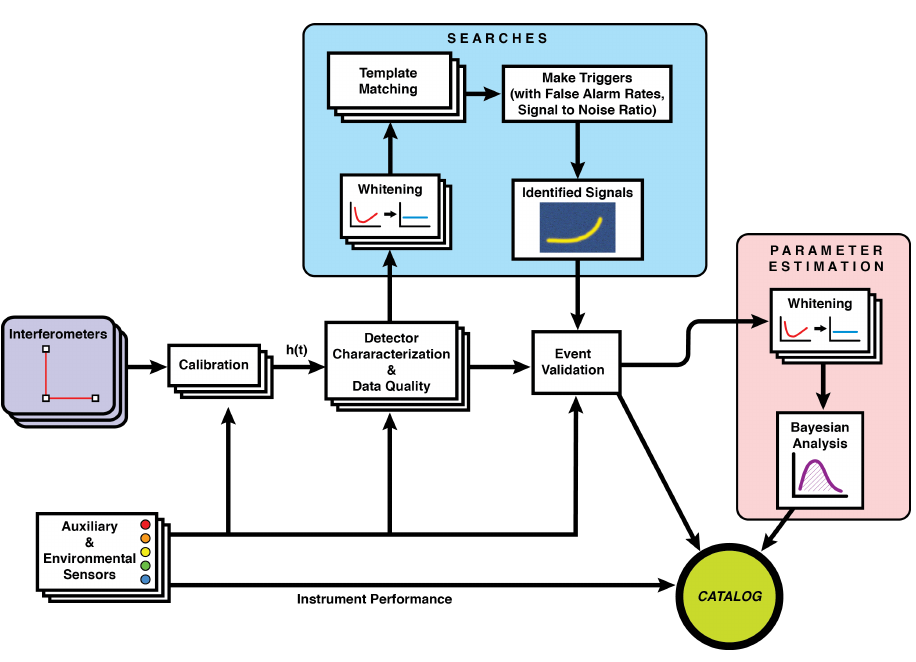
\includegraphics[width=\textwidth]{img/1_introduction/data_processing.png}
  \caption{asd}
  \label{fig:1_data_processing}
  \centering
\end{figure}



